\documentclass{llncs}
\usepackage{makeidx}
\usepackage{graphicx}
\bibliographystyle{splncs03}
\begin{document}
\title{Affectively Adaptive Level Generation for Mario}
\author{Peter Lehim Pedersen (pleh@itu.dk) \\Christoffer Holmg{\aa}rd Pedersen (holmgard@itu.dk)}
\institute{Procedural Content Generation in Games, Fall 2012}
\maketitle
\begin{abstract}
In this report, we describe the creation of a first emotionally adaptive level generation system for the Infinite Mario Framework. The system uses continuous physiological readings of sympathetic nervous activity (electrodermal activity and heart rate) as an expression of arousal from interacting with the game.
These arousal values are then tied to individual level elements, using an artificial neural network to learn individual players' dispositions toward specific level design elements and use this to procedurally generate personalized levels, predict the player's response and evaluate the actual response to the generated content.
\end{abstract}
\section{Introduction}
What does it mean for a game to be fun? Enjoyable? Good, even? The subjective experience of emotions related to (video) gameplay are hard to define, quantify and measure objectively.

One possibility is to try and infer the player's engagement with the game, or aspects thereof, and use this as one measure of the quality of the play experience.
Engagement can, in turn, with some reduction be operationalized into the player's emotional arousal; a unifying term for the relative sympathetic activation in an individual's nervous system at a particular time.

What in turn stimulates arousal in the player? One obvious answer would be the sum of events that take place over the course of a game, which in turn are unique to each particular game. For classic 2D platform games, the level of the game, in conjunction with the actions NPCs and the player, presents the primary predisposing configuration that determines which events will take place, and hence which level of arousal might be produced in the player.

For this project, we endeavored to create an adaptive level generator for the Infinite Mario Framework. The purpose of the adaptive level generator is to generate individualized levels that predispose the player's experience of a particular 'arousal curve', allowing a designer to predetermine the rise and fall of arousal over the course of a playthrough.

\section{Background and state of the art}
Arousal can be inferred from a multitude of behavioral and physiological signals - indeed the field of affective computing has it as a main goal to establish which channels and to which degree. Two of the most well-established signals in terms of usefulness for measuring arousal are electrodermal activity and heart rate varaibility [REFERENCE PICARD HERE]. 

These physiological signals can be obtained from a game player with relatively little intrusion upon the player and provide responsive measures of arousal that can be gathered in real time [REFERENCE HERE].

Professional game development studios have successfully used electrodermal activity and heart rate variability as measures of arousal and used the signals to provide input to 'AI directors' that manipulate the events of a game to influence player arousal, but only in laboratory settings.
A notable example is Valve's work on the Left 4 Dead 2 and Alien Swarm games, where in-game attacks from groups of enemies have successfully been timed to create a roller-coaster like experience of suspense.

Still, it would seem that the technology is not ready for deployment in commercial settings, even though some preliminary moves in that direction have been made by major console makers. In 2011 Sony several filed patents for controllers with embedded physiological measurement components and in 2009 Nintendo annouced the development of the Wii Vitality sensor; a peripheral for the Wii console with sensors for electrodermal activity and heart rate variability. Still, none of these products have reached the consumer market to date. This may indicate that the integration of the use of psychophysiological signals into hardware, and perhaps game design, remains a difficult project outside of controlled laboratory conditions and that more research is needed to provide robust and useful methods for using these signals in ways that are relevant for game design. Recent research does, however, indicate that this is an avenue that may be worth pursuing [REFERENCES HECTOR AND GEORGIOS HERE].

Using the data for guiding the procedural selection and generation of content (including, but not limited to event scheduling) for enabling player-adaptive games represents one such opportunity, which we decided to explore for this project.

\subsection{Game design}
The Infinite Mario Framework, is a game derivative of the highly succesful 2D sidescrolling platformer series, Super Mario Brothers. The game features a simplistic simulation of gravity that allows Mario to walk, run, and jump - and impressively move midair while in a jump! Using these abilities the object of the game is to guide the protagonist Mario through a level consisting of various obstacles and enemies.

All enemies exhibit simple, consistent behvioral patterns, bringing them close to being moving, deadly obstacles than NPCs proper. As such, the main determinant of the difficulty of any given play session is the configuration of the level.

Though the framework features a relatively small amount of obstacles and enemies to configure each level from, it allows for an practically infinite amount of variation though the placing of these elements and adjustement of the lengths of levels.

The original Super Mario Brothers games featured levels that were hand crafted by human level designers. This ensures a consistent experience for all players and graded diffuculty curve throughout the game, but does not take individual player skill or preference into account.

Since every level is configured by individual components, or tiles, provides a prime opportunity for using procedural content generation to support or replace the human designer.

\section{Methods}
The overall purpose of the bio-level-generator (BLG) that we constructed was to produce levels that were capable of inducing particular patterns of arousal in the player. The ambition was to predict what arousal a particular level feature would induce in a particular player and structure the sequence of features to provide a personal roller-coaster-ride of arousal through a particular level. Ultimately, the solution should allow a designer to specify nothing more than the curve of arousal that she would like the player to experience and the level should be generated adaptively.

For the current project we aimed to make our players have an experience illustrated by the curve in figure \ref{fig:ideal}. This was our ideal curve for the current version of the level generator and would serve as the later point of reference for the level generator.
\begin{figure}
\centering
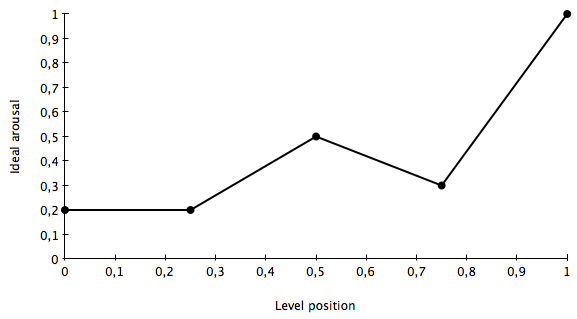
\includegraphics[scale=0.4]{idealGraph.png}
\caption{The intended - or ideal - arousal throughout the level}
\label{fig:ideal}
\end{figure}
Thus the challenge was to provide a mapping between level features and player arousal. To enable this, we produced an experimental setup where each player would play two levels. The first would serve as a benchmark for establishing the player's arousal reponse to different level features. The second would use this information to generate the adapted level.

\subsection{Screen-Chunks and Chunks}
In order to procedurally generate levels for Mario we needed a method for configuring individual tiles into levels in a way that would motivate gameplay with varying degrees of complexity, with the underlying assumption that this would lead to varying degress of difficulty and hence engagement and arousal.

Though levels are fundamentally configured of tiles, the individual tile is not necessarily the best level for describing the challenges that the player faces in the game. A tile is quickly traversed by Mario, and the difficulty of doing so can only be determined by looking at neighboring tiles.

Therefore, we decided to understand particular configuration of tiles, or chunks of tiles, as the fundamental unit of challenges that the player faces in the game. The guiding principle for defining a chunk was to look at configurations of tiles that necessitate the player to perform one action, or one combination of actions, to traverse the configuration: for instance jumping over a gap, or onto an enemy to kill it.

Additionally, we defined the concept of screen-chunks: configurations of chunks that are close enough for the actions connected to the chunks to influence each other: E.g a jump over one chunk making Mario land near an enemy that he must kill or avoid.

The fundamental principle of procedurally constructing a level was to connect screen-chunks until a desired level width was achieved. For each screen-chunk, windows for Mario's entry and exit were defined. The windows were required to overlap in neighboring screen-chunks.

The chunks and screen-chunks were designed manually with a custom editor and compiled into a screen-chunk library. It fell to the human designer to ensure that chunks and screen-chunks were passable by the rules of the game. During the design process we tried to ensure a varity of complexity and difficulty in the library, though these evaluations were only based on the expertise of the designer.

Each screen-chunk had a related weight that represented its assumed potential for generating arousal. For random levels this was ignored, while for adapted levels, this was used to select the order of screen-chunks.

\subsubsection{Generating Screen-Chunk Weights}
During playthrough of randomly generated levels, arousal responses (as expressed by skin conductivity levels from the player were continuosly sampled at a rate of 30Hz, and mapped to the corresponding screen-chunks.

Before any attempts at adaptivity were done, two reference players were asked to play through a miltutude of randomly generated levels, constructing a dataset of 490 observations of arousal responses to screen-chunks distributed across the library. [INDSÆT INFO HER, HVIS VI GIDER] The observations were then used to train an artificial neural network regressor to predict arousal values for the individual screen-chunks in the library.

For sessions featuring adaptivity, further, personal, observations were gathered from the first playthrough of a random level. Then, they were used to further train the ANN from it's baseline state toward a personalized state.

Finally, this new adapted ANN was used to predict personal weights for every screen-chunk in the library. This updated library then formed the basis for generating personal, adapted levels.

\subsubsection{SCL sampling and treatment}
Preliminary work for the experiments was done using a wireless physiological measurement device called the Empatica E2.
However, we experienced device failure over the course of the project and subsequently psychophysiological sampling was conducted with a Wild Divine Lightstone Biofeedback device which connects via USB.

The Lighstone device is capable of sampling skin conductivity levels and blood volume pulse at a rate of 30Hz. Samples were taken from the three leftmost fingertips of the player's left hand. The controls of the Mario game were adapted to minimize the incovenience of wearing the Lightstone while playing. 

Using the publicly available jlsm software package [reference here], we constructed  custom sampling functionality that allowed us for fusing real-time sample data with real-time gameplay data from the Mario Framework.

Signals were sampled at the maximum rate available (30Hz). Before play start, the player went through a 30s period of baseline measurement viewing a blue screen with a countdown. Once the level started, each sample was tagged with the horisontal position of Mario in the level at sample time. 

Though we were not able to precisely measure the latency from device sampling to in-game location mapping we assumed this to be low enough to be neglible. The width of the screenchunks allowed us to assume that most skin conductivity responses to in-game events, in a given screen, would be mapped to the response eleciting screen-chunk.

After the playthrough, the raw samples from of SCL levels were subjected to smoothing by a simple moving average to remove noise from signal. The full signal, including the baseline, was then scaled to values between 0 and 1. Subsequently the mean SCL value for each screenchunk in the level was calculated, as well as the maximum value measured during time spent in that screen chunk.

Finally, for each screenchunk that the player had experienced in the level, an observation was generated. Each observation consisted of the count of individual chunks in the screen-chunk, and the mean SCL value. These observations were then used as training examples for the ANN regressor, that in turn would be used to predict screen-chunk arousal induction potential.

\subsection{Results}
A number of network topologies were attempted. The best performing one was a 3-2 hidden layer topology, trained for 100.000 epochs. The ANN regressor exhibited a correlation coefficient of 0,3122 between expected an produced values and a relative absolute error of ca. 89\%. Though this performance was slightly discouragning, we proceeded to use the network for a pilot run of four user tests.
Two of these players did not manage to complete the personalized levels, arguably because the generated level was unfit for their skill level.
The two other players completed their personalized levels. Their arousal responses to the random and personalized levels are included in in figures \ref{fig:playerFirst} and \ref{fig:playerLast}.

Since it was impossible to, within the scope of this project, to collect a data material suitable for extensive stastiscal analysis, we instead opted to present these preliminary results on a case-by-case basis.

For the method to be considered succesful for this first pilot-run, we would require the curves of the personalized sessions to conform, at least to some extent, to the chosen ideal curve presented earlier in figure \ref{fig:ideal}.

While none of the signals correspond clearly to the curve we tried to induce, we find it worth noticing that both players exhibit spikes of arousal activity at the middle of the level, followed by drops in arousal, which are then followed by a second spike in activity at the end of the personalized level. However, we also see patterns of spikes completely seemingly unrelated to the desired arousal curve.

\begin{figure}
\centering
\includegraphics[scale=0.4]{movieStar.png}
\caption{Player I}
\label{fig:playerFirst}
\end{figure}
\begin{figure}
\centering
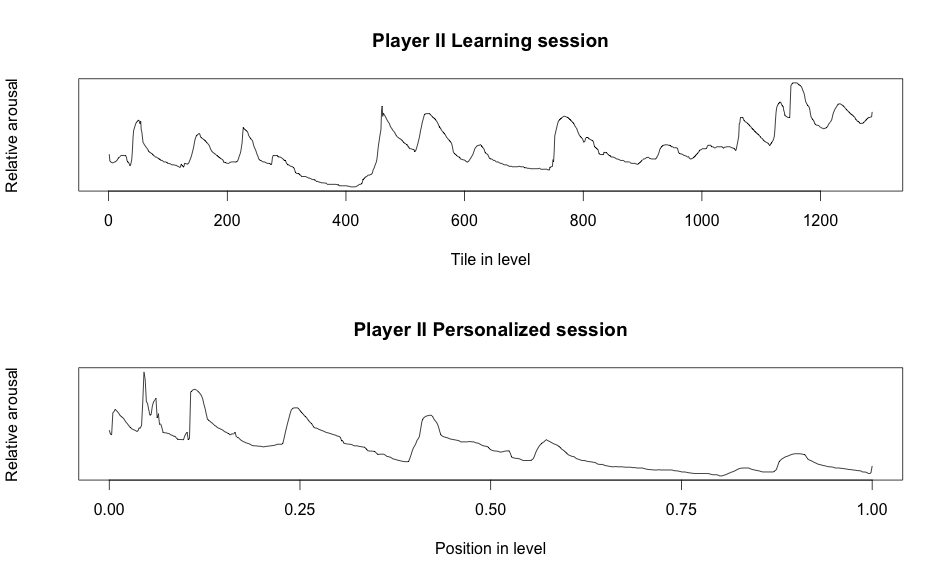
\includegraphics[scale=0.4]{nicklas.png}
\caption{Player II}
\label{fig:playerLast}
\end{figure}

\section{Discussion}



\subsubsection{Classification}
ifht. til sb-pcg  paper
Offline, necessary, parametrized(?), mix of stocahstic and deterministic, constructive (but based parameters from person)
\subsubsection{Arousal-engagement assumptions}
Is arousal the same thing as engagement - how do we discern between various kinds of arousal; we don't!
\subsubsection{Signal noise}
Movement artifacts
\subsubsection{Response lag/screen chunk width}
How long time does a response time. How long is drop-off of response.
\subsubsection{Habituation/player learning}
Skill, learning rate, fatigue
\subsubsection{Player characteristics}
Skill, day dependence, relevance of base model, 

\section{Conclusion and future work}
Some indications of correlation between expected responses and actual responses.

Some problems in the paradigm.

Insufficient number of observations in the dataset.

More screenshunks would be preferable, but ties in with the size of the dataset.

More advanced signal analysis; that can still run between individual play sessions! (

Need s to be quick; is machine learning an option, really?)

Is this a feasible way of doing PCG? Not commercially yet - will it ever be?

Real-time learning and generation

\bibliography{references}
\end{document}